\documentclass[11pt, oneside]{article}   	% use "amsart" instead of "article" for AMSLaTeX format
\usepackage[left=1.5in, right=1.5in, top=1in, bottom=1.5in]{geometry}                		% See geometry.pdf to learn the layout options. There are lots.
\geometry{letterpaper}                   		% ... or a4paper or a5paper or ... 
%\geometry{landscape}                		% Activate for rotated page geometry
%\usepackage[parfill]{parskip}    		% Activate to begin paragraphs with an empty line rather than an indent
\usepackage{graphicx}				% Use pdf, png, jpg, or eps§ with pdflatex; use eps in DVI mode
								% TeX will automatically convert eps --> pdf in pdflatex		
\usepackage{amssymb}
\usepackage{caption}
\usepackage{hyperref}
\usepackage{braket}
\usepackage{amsmath}
\usepackage{setspace}  % For custom line spacing
\usepackage{enumitem} % For customizing list styles

%SetFonts

\setstretch{1.26}  % Change the value here to control the line spacing

%SetFonts


\title{Enhancing Fraud Detection with Quantum Machine Learning: A Comparative Study of Quantum and Classical Approaches}	
\author{}
\date{2024-10-25}							% Activate to display a given date or no date

\begin{document}
\maketitle


% -----------------------------------------------------------Abstract-------------------------------------------------------------------------------------------------


\begin{abstract}
Include abstract once results are finalized...
\end{abstract}


% -----------------------------------------------------------Introduction-------------------------------------------------------------------------------------------------


\section{Introduction}

\hspace{10mm}Recent years have seen groundbreaking research in both machine learning and quantum computing, positioning these fields at the forefront of some of the most anticipated scientific breakthroughs. Quantum computers promise to solve problems once deemed unsolvable by classical computing, while advancements in generative AI are poised to spark the next major technological revolution, with tech companies racing to develop and deploy their own AI-driven solutions. While much of the excitement around each field has largely remained within their respective domains, researchers have been able to combine components of each to create what are known as quantum machine learning (QML) models. QML combines the processing power of quantum computing with existing machine learning models in an effort to theoretically optimize both their performance.\\

\noindent\hspace{10mm}The work presented here showcases how QML can be used to predict credit card fraud as an example of its potential fraud detection capabilities. Fraud detection has become an increasingly important area of research in recent years, given that the methodologies utilized by fraudsters are continuously evolving in complexity, posing novel challenges that push the limits of traditional detection systems. As such, QML can be a possible solution to fight back against these increasingly sophisticated fraudulent attacks. \\

\noindent\hspace{10mm}Using IBM’s \texttt{qiskit} Python library, various aspects of simulated quantum circuits were examined in order to model how different system parameters affected the results of the QML algorithms that they implemented. These circuits were then used to encode classical data into a quantum feature space, and ingested by machine learning algorithms that could predict the presence of fraud in credit card transactions. These results were then compared to those generated using classical data. This project focuses on two ML algorithms in particular - Support Vector Machines (SVM) and Random Forests (RF) - along with their QML counterparts - Quantum Support Vector Machines (QSVM) and Quantum Random Forests (QRF). 


% ----------------------------------------------------------Literature Review--------------------------------------------------------------------------------------------------


\section{Literature Review}

\noindent\hspace{10mm}While being a relatively new field, QML has still seen a number of groundbreaking developments over the years that demonstrate how quantum mechanics can be adapted to tackle complex data processing tasks. Using quantum computers to solve classification problems was explored as early as the late 1990's, in which \href{https://journals.aps.org/pra/abstract/10.1103/PhysRevA.58.915}{Farhi et al. (1998)} theorized how quantum computers could be used to build decision tress [\href{https://journals.aps.org/pra/abstract/10.1103/PhysRevA.58.915}{1}]. Later, \href{https://arxiv.org/abs/1907.06840}{Khadiev et al. (2019)} showed how using Grover's algorithm (also known as the quantum search algorithm) could be exploited to improve the efficacy of quantum decision trees, laying the groundwork for their team to be able to eventually demonstrate how to build QRFs in practice \href{https://arxiv.org/abs/2112.13346}{(Khadiev et al. (2021)} [\href{https://arxiv.org/abs/1907.06840}{2}, \href{https://arxiv.org/abs/2112.13346}{3}]. Most recently, QRFs that utilize ``quantum kernels" have been shown to further enhance their ability to process and analyze data, first evidenced by \href{https://arxiv.org/abs/2210.02355}{Srikumar et al. (2022)} [4]. \\

\noindent\hspace{10mm}Research on how to apply quantum enhancements to machine learning has been extended to numerous additional algorithms, including support vector machines (SVMs). In the early 2000s \href{https://members.cbio.mines-paristech.fr/~jvert/svn/bibli/local/Anguita2003Quantum.pdf}{Anguita et al. (2003)} first laid out the theoretical foundation for how quantum computing could be use to train SVM models [\href{https://doi.org/10.1016/S0893-6080(03)00087-X}{5}]. \href{https://arxiv.org/abs/1307.0471}{Rebentrost et al. (2014)} and \href{https://doi.org/10.26421/QIC17.15-16}{Chatterjee et al. (2017)} expanded on this early work to show how QSVMs could be produced in practice by creating quantum versions of the kernel needed by SVM models to transform data into a higher dimensional space [6]. 

\noindent\hspace{10mm} While many other theory-based papers were identified over the course of this literature review, the following comprehensive studies provide brilliant summaries of the numerous techniques and developments seen over the course of QML's relatively brief history: 

\begin{itemize}

\item \href{https://doi.org/10.1038/nature23474}{Biamonte et al. (2017)} provides a robust review of the theoretical framework behind QSVM and the potential benefits that can be achieved when compared to using traditional SVMs [\href{https://doi.org/10.1038/nature23474}{7}]. 
\item \href{https://pubmed.ncbi.nlm.nih.gov/36832654/}{Zeguendry et al. (2023)} provides a concise overview of the quantum mechanics involved in building QML algorithms and provides numerous case studies of how these algorithms can be applied in practice [\href{https://doi.org/10.3390/e25020287}{8}]. 


\end{itemize}

\noindent\hspace{10mm}Each of the above papers have numerous citations and were used as key points of reference while completing the work presented here. \\

\noindent\hspace{10mm}There are also numerous instances of instances in which QML algorithms are applied to real world scenarios to test the potential upsides speculated in the aforementioned theoretical research. The list below includes some noteworthy examples: 

\begin{itemize}

	\item \href{https://doi.org/10.21203/rs.3.rs-1434074/v1}{Shan et al. (2022)} used QSVMs as a methodology for breast cancer detection and show that it can match accuracy results comparable to that of classical SVMs [\href{https://doi.org/10.21203/rs.3.rs-1434074/v1}{9}].
	\item \href{https://doi.org/10.48550/arXiv.2408.04543}{Luo et al. (2024)} have shown that QML algorithms have ``promising potential" when being used to predict predict the presence of Alzheimer's disease, though have not yet surpassed their classical counterparts in terms of learning capability [\href{https://doi.org/10.48550/arXiv.2408.04543}{10}].  
	\item \href{https://doi.org/10.22331/q-2023-11-29-1191}{Cherrat et al. (2023)} were able to develop a reinforcement learning model via Quantum Neural Networks (QNNs) and used financial sector data to tackle the problem of hedging [\href{https://doi.org/10.22331/q-2023-11-29-1191}{11}]. 

\end{itemize}

\noindent\hspace{10mm}Numerous additional case studies of QML are summarized in a study done by \href{https://doi.org/10.34190/eccws.23.1.2258}{Nguyen et al. (2024)}, which draws on the findings from 32 previously written papers in the field that give a robust summary of the potential upside that can be realized when switching to use QML algorithms [\href{https://doi.org/10.34190/eccws.23.1.2258}{12}]. This paper was also used as a consistent point of reference when completing the work presented here. A review of these numerous case studies reveals that QML algorithms either very nearly approach of exceed the performance seen from classical ML algorithms, fostering excitement when considering the prospect of applying these findings specifically to the realm of fraud detection. \\

\noindent\hspace{10mm}That being said, there is already some existing work that shows how quantum machine learning can be used in fraud detection problems. Namely, \href{https://doi.org/10.1142/S0219749923500442}{Innan et al. 2023} demonstrates that QSVMs seem to outperform Quantum Neural Network (QNN) algorithms when solving fraud detection problems, while \href{https://arxiv.org/abs/2208.01203}{Kyriienko et al. (2022)} show that QSVMs have similar performance compared to classical SVMs when trying to identify fraudulent banking transactions [\href{https://doi.org/10.1142/S0219749923500442}{13}, \href{https://doi.org/10.48550/arXiv.2208.01203}{14}]. That being said, the purpose of this work is to extend beyond the existing research to specifically quantify how changing the features of a quantum circuit affect the results of both the and QSVM and QRF algorithms in regards to predicting credit card fraud, and compare the results of \textit{both} algorithms against those of their classical counterparts.\\

\noindent\hspace{10mm}It is worth noting that as of July 2024, it has been revealed that Deloitte is exploring using QML (specifically, QNNs) to detect fraudulent online payments [\href{https://thequantuminsider.com/2024/07/19/deloitte-italy-explores-quantum-machine-learning-for-digital-payments-fraud-detection/}{15}]. While they have provided no study of their results, the work presented here could provide quantitative evidence that utilizing QML should be considered as a possible next step in the ongoing fight against fraud. 


% -------------------------------------------------------------Hypothesis-------------------------------------------------------------------------------------------


\section{Hypothesis}

Given the findings of the literature review, it appears clear that QSVMs should approach or exceed the performance of a classical SVM model in identifying credit card fraud, especially after the best quantum circuit for the scenario has been identified. Given the arguably superior ability of RFs over SVMs to handle high dimensional feature spaces, it is expected that QRFs should be able to build on the gains realized by QSVMs. Once again, this is only after the best tuned quantum circuit has been identified. Identifying these ideal quantum circuits, will be an exercise in balancing complexity: adding to the circuit's ability to handle more complex data structures (by increasing the number of qubits, using more expansive entanglement patterns etc.) will likely increase model performance up a point, but will eventually witness decreased efficiency and suffer from added noise. 


% -----------------------------------------------------------Data----------------------------------------------------------------------------------------------------


\section{Data}
\subsection{Data Source}

\hspace{10mm}The dataset used in this project is sourced from Kaggle and contains data of over 550,000 credit card transactions in the EU during 2023 [\href{https://www.kaggle.com/datasets/nelgiriyewithana/credit-card-fraud-detection-dataset-2023}{16}]. The original source of the data is the result of a research collaboration between Worldline and the Machine Learning Group of ULB (Université Libre de Bruxelles) ]\href{https://www.researchgate.net/publication/283349138_Calibrating_Probability_with_Undersampling_for_Unbalanced_Classification}{17}]. The data is anonymized to protect the identity of the credit card users and contains 29 predictor variables representing various aspects of each credit card transaction.  Due to the anonymization, it is impossible to know exactly what each of these first 28 features represent (they are all labelled simply as V1 through V28), but it is shared that they represent the commonly captured features of a credit card transaction (i.e. time, location, etc.). These first 28 features have all been transformed to be continuous numerical features. The only titled predictor variable in the dataset is ``Amount", which represents the total amount of the credit card transaction in Euros. The goal when using this dataset will be to predict ``Class”, a binary field indicating whether or not the transaction was fraudulent.

\subsection{Data Cleaning}

\hspace{10mm}Datasets for this project were considered only if they had a reputation for being clean and usable, ensuring the focus remains on model performance rather than being heavily influenced by data cleaning, imputation, or collection methods. As such, this dataset contains 568,630 records in which none of the fields have missing, misprinted, or nan values. The target variable, ``Class", contains either 1 or 0, indicating whether the observation is fraudulent (1) or valid (0). \\
	

% ------------------------------------------------------------Methods----------------------------------------------------------------------------------------------------


\section{Methods}


% ------------------------------------------------------------Methods: Data Sampling------------------------------------------------------------------------------------------------


\subsection{Data Sampling}

As previously mentioned, the chosen dataset contains over half a million observations. Given the computational complexity of fitting certain models to a dataset of this size, a vast reduction in the number of samples was warranted. Additionally, Figure 1 highlights an additional complication with the original dataset: balanced classes. 

\begin{figure}[h!]
    \centering
    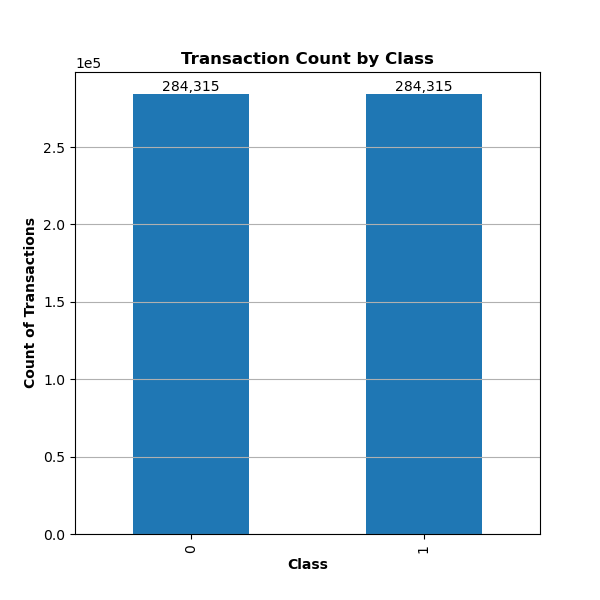
\includegraphics[width=0.6\textwidth]{figures/fig_1.png}
    \captionsetup{font=small} 
    \caption{There are an equal number of fraudulent (1) and valid (0) transactions in the initial dataset.}
    \label{fig1}
\end{figure}

Though the balanced dataset might make it easier to predict instances of fraud, it is not representative of what would occur in the real world. The European Banking Authority (EBA) estimates that ``fraud accounted for 0.031\% of total card payments in value and 0.015\% of total card payments in volume terms in H1 2023" [\href{https://www.eba.europa.eu/sites/default/files/2024-08/465e3044-4773-4e9d-8ca8-b1cd031295fc/EBA_ECB\%202024\%20Report\%20on\%20Payment\%20Fraud.pdf}{18}]. To combat both of these issues the following took place place:

\begin{enumerate}
	\item{Sample the dataset so that only 1\% of observations represent fraudulent transactions.}
	\item{Only include 10,000 observations in total.}
\end{enumerate}

To do this, 100 class 1 samples and 9,900 class 0 samples were randomly selected from the original dataset, without replacement. These subsets were then combined forming a new sampled dataset to use for analysis and modeling. Although the percentage of fraudulent transactions is still inflated compared to the estimate made by the EBA, this update shifts the machine learning objective to actual fraud detection while ensuring that a sufficient number of fraudulent samples are retained. Figure 2 shows the the updated version of transactions by class after the change.\\

\begin{figure}[h!]
    \centering
    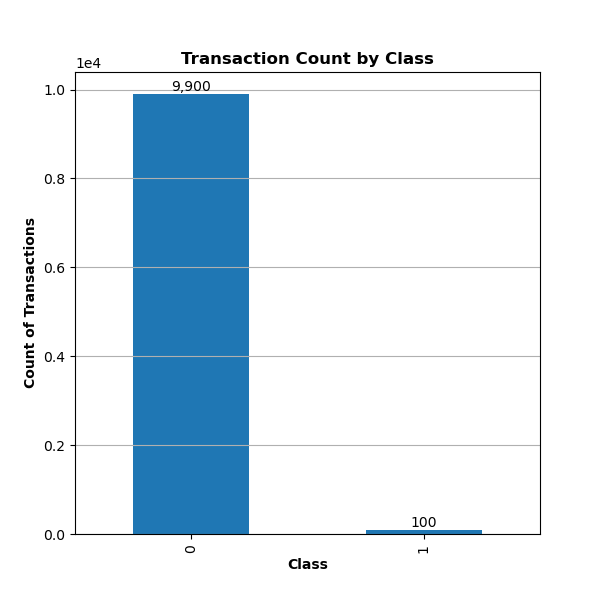
\includegraphics[width=0.6\textwidth]{figures/fig_2.png}
    \captionsetup{font=small} 
    \caption{The updated breakdown by class represents a paints a more realistic picture of credit card fraud, and still maintains a large number of transactions.}
    \label{fig2}
\end{figure}


% ------------------------------------------------------------Methods: Data Preprocessing------------------------------------------------------------------------------------------------


\subsection{Data Preprocessing}


% ------------------------------------------------------------Methods: Data Preprocessing: Outliers------------------------------------------------------------------------------------------------


\subsubsection{Outliers}

An outlier analysis was performed in which outliers present within each predictor field were identified via well established Tukey's method [\href{https://books.google.com/books/about/Exploratory_Data_Analysis.html?id=UT9dAAAAIAAJ}{18}]: 

Given a vector $X$, a data point $x_i \in X$ is considered an outlier if it satisfies:
\begin{equation}
x_i < Q_1 - 1.5 \cdot \text{IQR} \quad \text{or} \quad x_i > Q_3 + 1.5 \cdot \text{IQR}
\end{equation}

such that $Q1$ and $Q3$ represent the first and third quartiles of $X$, and $\text{IQR} = Q_3 - Q_1$ (the inter-quartile-range of $X$). Figure 3 shows the results of this analysis:

\begin{figure}[h!]
    \centering
    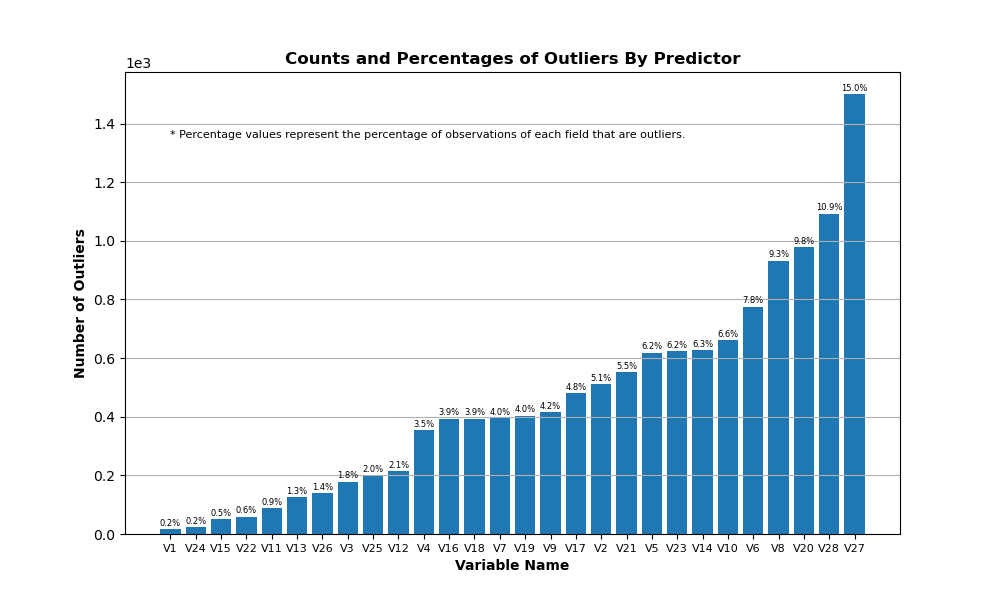
\includegraphics[width=1.0\textwidth]{figures/fig_3.png}
    \captionsetup{font=small} 
    \caption{Outliers are present in each of the predictor variables when using the definition from Equation 1. Some fields having enough to comprise greater than 10\% of their total observations.}
    \label{fig3}
\end{figure}

To reduce the quantity of outliers in the data and mitigate any potential negative impacts they might have when attempting to fit models, a Windsorization transformation was applied to the data [\href{https://doi.org/10.1214/aoms/1177730388}{19}]. Winsorization is a statistical transformation technique used to limit extreme values in a dataset by replacing them with specified percentiles and is defined as follows:

Given a vector $X$, a data point $x_i \in X$, and chosen percentiles $p_{\text{max}}$ and $p_{\text{min}}$, let $x_{\text{max}}$ and  $x_{\text{min}}$ represent the values at each of the chosen percentiles. Windsorization transforms $x_i \rightarrow x_i'$ via:

 
\begin{equation}
x_i' = 
\begin{cases} 
x_i, & \text{if }  x_{\text{min}} \leq x_i \leq  x_{\text{max}} \\
x_{\text{min}}, & \text{if } x_i <  x_{\text{min}} \\
x_{\text{max}}, & \text{if } x_i >  x_{\text{max}}
\end{cases}
\end{equation}

This transformation ensures that values below the $p_{\text{min}}$-th percentile are replaced by $x_{\text{min}}$, and values above the $p_{\text{max}}$-th percentile are replaced by $x_{\text{max}}$. In this instance, the 5th and 95th percentiles were chosen as the limits of the Windsorization transformation. \\


% ------------------------------------------------------------Methods: Data Preprocessing: Normality------------------------------------------------------------------------------------------------


\subsubsection{Normality}

To determine if the data present in each of the predictor fields followed a gaussian distribution the $\texttt{normaltest}$ function from Python's $\texttt{scipy.stats}$ library was used [\href{https://www.nature.com/articles/s41592-019-0686-2}{20}]. The implementation is based on D'Agostino and Pearson's test omnibus test that combines skewness and kurtosis to produce an omnibus test of normality[\href{https://doi.org/10.2307/2334522}{21}, \href{https://doi.org/10.2307/2335012}{22}]. The null and alternative hypotheses for the test are as follows:

\begin{align}
H_0 &: \text{Data follows a normal distribution.} \\
H_a &: \text{Data does not follow a normal distribution.}
\end{align}


Applying this test to each of the predictor fields resulted in $p$-values $<$ 0.05 meaning that we can reject the null hypothesis and consider the data as non-normal. In an effort to address this (and also possibly further limit the influence of the previously identified outliers), a Yeo-Johnson power transformation was applied (Box-Cox was not considered due to the presence of negative values in the dataset) [\href{https://doi.org/10.1093/biomet/87.4.954}{23}]. A definition of this transformation is given below:

Given $x_i \in X$ and a transformation parameter $\lambda$, the Yeo-Johnson transformation maps $x_i \to x_i' $ via:

\begin{equation}
x_i' =
\begin{cases} 
\frac{(x_i + 1)^\lambda - 1}{\lambda}, & \text{if } x_i \geq 0 \text{ and } \lambda \neq 0, \\
\log(x_i + 1), & \text{if } x_i \geq 0 \text{ and } \lambda = 0, \\
-\frac{(-x_i + 1)^{2 - \lambda} - 1}{2 - \lambda}, & \text{if } x_i < 0 \text{ and } \lambda \neq 2, \\
-\log(-x_i + 1), & \text{if } x_i < 0 \text{ and } \lambda = 2.
\end{cases}
\end{equation}

$ \lambda$ in this case is determined when running the $\texttt{normaltest}$ function, and is the value that maximizes the normality of the transformed data. 


% ------------------------------------------------------------Methods: Data Preprocessing: Multicollinearity------------------------------------------------------------------------------------------------


\subsubsection{Multicollinearity}

Figure 4 shows a correlation matrix of the dataset, which highlights the correlations between all pairs of predictor variables. 

\begin{figure}[h!]
    \centering
    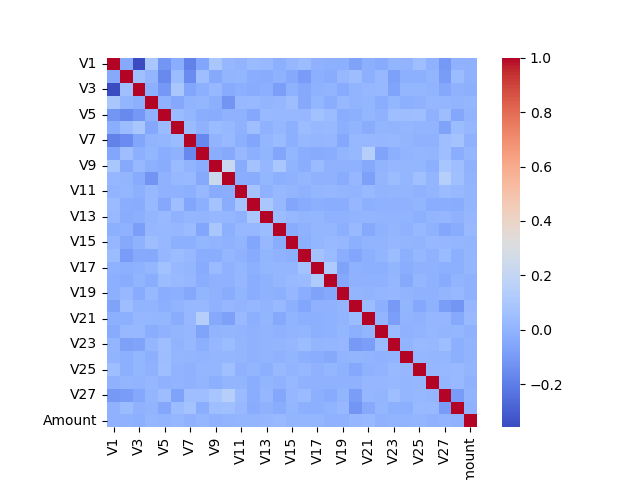
\includegraphics[width=1.0\textwidth]{figures/fig_4.png}
    \captionsetup{font=small} 
    \caption{A correlation matrix of the transactions dataset. All correlations $r$ were within $-0.36 < r < 0.23$.}
    \label{fig4}
\end{figure}

Visual inspection of the correlation matrix reveals that no pair of unique predictor variables maintain a troublesome degree of correlation, providing evidence for the fact that any dimensionality reduction transformations (i.e. PCA) are not necessary. 


% ------------------------------------------------------------Methods: Data Preprocessing: Scaling------------------------------------------------------------------------------------------------


\subsubsection{Scaling}

Given that the data was not originally considered normal, standard scaling (in which $\mu$=0 and $\sigma=1$ is not appropriate. Additionally, min-max scaling (which scales all values to lie between 0 and 1) is highly sensitive to outliers, making it unsuitable for this case. Robust scaling, on the other hand, is a preferred approach when handling data with outliers [\href{https://books.google.com/books/about/Exploratory_Data_Analysis.html?id=UT9dAAAAIAAJ}{18}]. It centers each field around its median and scales it based on its interquartile range (IQR), effectively minimizing the influence of extreme values. As such, this was the scaling transformation applied in this case. A definition of robust scaling is provided below:

Given \( x_i \in X \), robust scaling transforms \( x_i \to x_i' \) via:

\begin{equation}
x_i' = \frac{x_i - Q_2}{\text{IQR}}
\end{equation}

where $Q_2 $ and \text{IQR} are the median of  and inter-quartile-range of $ X$, respectively.


% ------------------------------------------------------------Methods: Data Preprocessing: Full Transformation Pipeline---------------------------------------------------------------------------------------------


\subsubsection{Full Transformation Pipeline}

In summary, the following data pre-processing were applied to the dataset.

\begin{enumerate}
	\item Split the data into testing and training sets. 25\% of the sample was kept for testing, with the proportion of classes being kept the same across both sets.
	\item Fit and apply Windsorization transformation to the training set.
	\item Use the fitted percentile values from step 2 to apply a Winsorization transformation to the testing set.
	\item Fit and apply Yeo-Johnson transformation to the training set.
	\item Use the fitted $\lambda$ value from step 4 to to apply a Yeo-Johnson transformation to the testing set.
	\item Fit and apply a robust scaling transformation to the training set.
	\item Use the fitted median and IQR values from step 6 to apply a robust scaling transformation to the testing set.
\end{enumerate}

The parameters used for each transformation are only determined via the training data in order to prevent data leakage. Figures 5 and 6 use box-plots to highlight the positive changes these transformations had on the distributions of the predictor variables. 

\begin{figure}[h!]
    \centering
    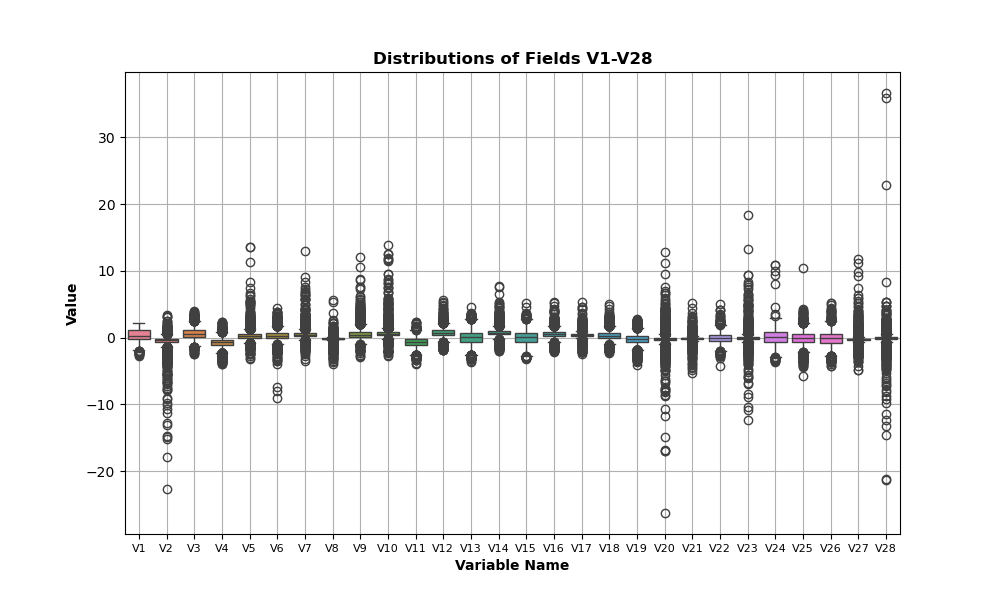
\includegraphics[width=1.0\textwidth]{figures/fig_5.png}
    \captionsetup{font=small} 
    \caption{Represents the data before any pre-processing transformations. The predictors suffer from varying distributions, ranges, and exhibit a large number of outliers.}
    \label{fig5}
\end{figure}

\begin{figure}[h!]
    \centering
    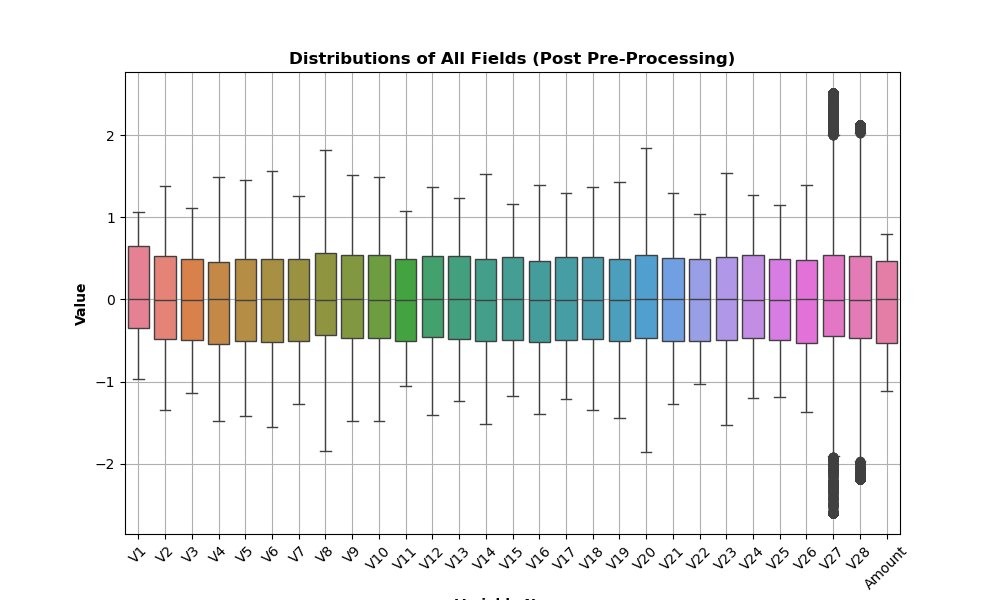
\includegraphics[width=1.0\textwidth]{figures/fig_6.png}
    \captionsetup{font=small} 
    \caption{Represent the data after all data pre-processing transformations. All but two fields now have outliers, and the range of their distributions no longer vary from one another.}
    \label{fig6}
\end{figure}


% ------------------------------------------------------------Methods: Exploratory Data Analysis------------------------------------------------------------------------------------------------


\subsection{Exploratory Data Analysis}

Before applying any machine learning models to the data, an initial analysis was completed in an effort to determine which of the explanatory variables might be useful in making predictions. To do this, $t$-tests were performed that compared the difference of means for each field when separated by class [\href{https://doi.org/10.2307/2331554}{24}]. Figure 7 shows the results of these $t$-tests, which show that many of the explanatory fields exhibited statistically significant differences when comparing the means of each variable by class.

\begin{figure}[h!]
    \centering
    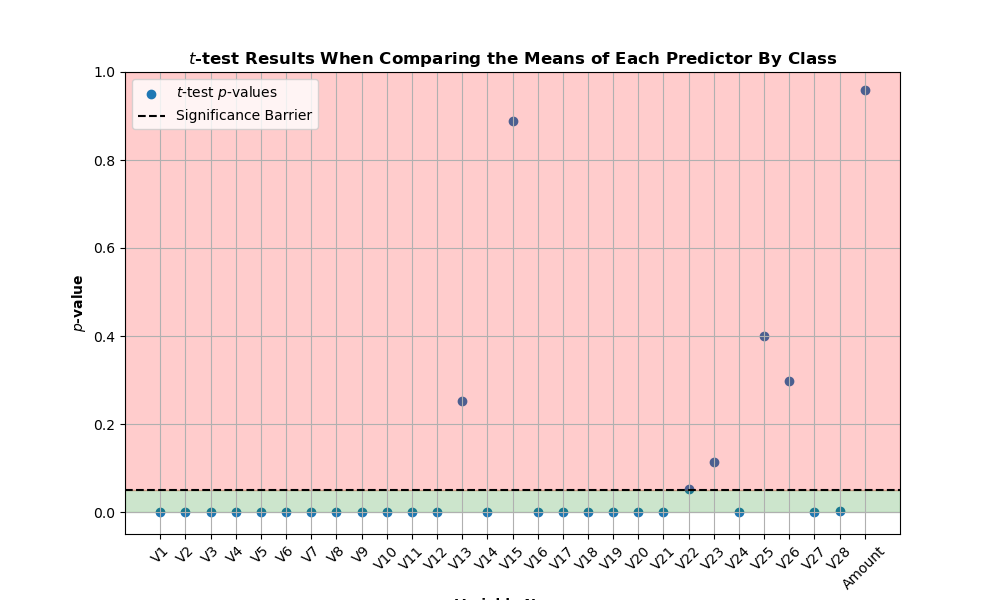
\includegraphics[width=1.0\textwidth]{figures/fig_7.png}
    \captionsetup{font=small} 
    \caption{Many of the predictor variables exhibit statistically significant differences when comparing the means of each class.}
    \label{fig7}
\end{figure}

Indeed, Figure 8 uses the V1 field as an example to show that a comparison of the distributions by class reveals a stark difference.

\begin{figure}[h!]
    \centering
    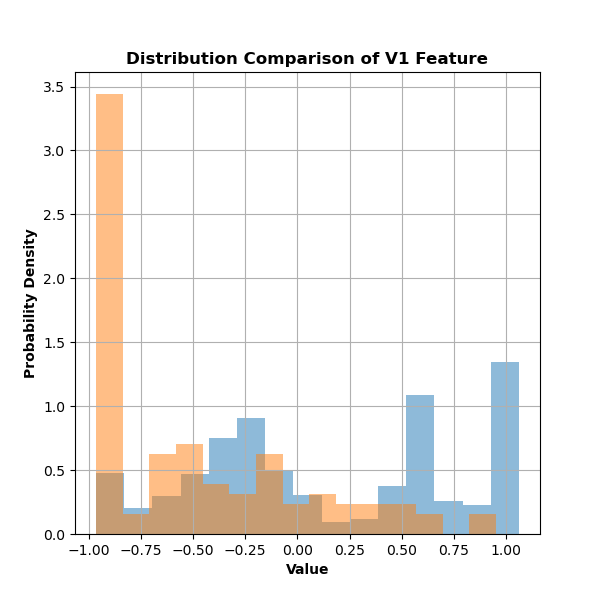
\includegraphics[width=0.6\textwidth]{figures/fig_8.png}
    \captionsetup{font=small} 
    \caption{V1 was one of the statistically significant field identified in Figure 7. The distributions completely different when comparing the two classes.}
    \label{fig8}
\end{figure}

This results of this analysis bode well for the quality of this dataset, as it appears to contain features that will be useful in making predictions on the target variable. It provides confidence that identifying the fraudulent transactions via ML algorithms is possible.


% ------------------------------------------------------------Methods: Classical ML Algorithms------------------------------------------------------------------------------------------------


\subsection{Classical ML Algorithms}

\hspace{10mm}

% ------------------------------------------------------------Methods: Classical ML Algorithms: Support Vector Machines-------------------------------------------------------------------------------------------


\subsubsection{Support Vector Machines (SVM)}

\hspace{10mm}Support Vector Machines (SVM) are a type of supervised learning algorithm used for classification tasks, especially when the data is not linearly separable [\href{https://link.springer.com/book/10.1007/978-1-4757-3264-1}{25}. The key idea behind SVM is to find the hyperplane that best separates the data into different classes. More specifically, SVM attempts to find the hyperplane that maximizes what's known as the \textit{margin} - the distance between the hyperplane and the nearest data points from each class (these distances are the ``support vectors"). In a simple two-dimensional space, this hyperplane is essentially a line that divides the data points, but in higher-dimensional spaces, it becomes a complex multidimensional boundary. Once the best hyperplane is identified, the SVM classifier can use this boundary to classify new data points.\\

\noindent\hspace{10mm}SVMs are a classic option when solving classification problems, and was one of the first to be adapted to be used on quantum computers according to the literature review. Consequently, they emerged as a clear choice when determining which ML algorithms to evaluate in this project. \\

SVM models consist of a number of tunable hyperparameters, such as:

\begin{itemize}
    \item \textbf{Kernel Type:} The function used to transform the data into a higher-dimensional space where it is more likely for the classes to be separable. Different types of kernels work well for different applications. For example, linear kernels work best when data is linearly separable in higher-dimensional space, while radial basis function (RBF) kernels work well for data with complex, non-linear patterns.
    \item \textbf{$C$:} A regularization parameter that affects the shape of the decision boundary. Higher $C$ values focus more on correctly classifying every observation in the training data, resulting in more complex decision boundaries that can lead to overfitting. Lower $C$ values allow for more misclassifications on the training data, resulting in a more generalized decision boundary that can potentially underfit the data.
    \item \textbf{$\gamma$:} This parameter is only required when using a radial basis function (RBF) kernel. $\gamma$ controls how far the influence of a single training point extends. Low $\gamma$ values capture broader patterns with smooth decision boundaries (risking underfitting), while high $\gamma$ values focus on local details (risking overfitting).
\end{itemize}

The above parameters were all tuned when building the benchmark SVM algorithm used as a benchmark to evaluate the performance of its Quantum counterpart. The tuning was performed using a three-fold cross-validation with the following as candidates for each of the hyperparameters:

\begin{table}[h!]
    \centering
    \begin{tabular}{|c|c|}
        \hline
        \textbf{Hyperparameter} & \textbf{Candidates} \\ \hline
        Kernel Type & Linear, RBF \\ \hline
        $C$  & 0.1, 1, 10 \\ \hline
        $\gamma$ & 0.01, 0.1, 1 \\ \hline
    \end{tabular}
    \caption{The hyperparameter candidates for the classical SVM model.}
    \label{tab1}
\end{table}

Given the choice of hyperparameter candidates, $2 \cdot 3 \cdot 3 = 18$ models were tested resulting in 54 total fits after the three-fold cross validation. The models were all built using \texttt{scikit-learn}'s \texttt{SVC} class [\href{https://www.nature.com/articles/s41592-019-0686-2}{20}]. To address the high level of class imbalance, \texttt{SVC}'s \texttt{class\_weight} argument was set to \texttt{`balanced'}. Doing so creates weights $(w_1, w_0)$ for each class such that $C$ is scaled as $C \cdot w_1$ for class 1 and $C \cdot w_0$ for class 0. The \texttt{`balanced'} setting adjusts the weights so that they are inversely proportional to class frequencies in the input data, allowing the algorithm to account for class imbalance. More specifically:

The weight for class $c$, $w_c$ is calculated as:

\begin{equation}
w_c = \frac{N}{n_{\text{classes}}\cdot n_c}
\end{equation}

where $N$ = total number of observations, $n_c$ is the total number of observations of class  $c$, and $n_{\text{classes}}$ is the total number of classes. \\

Lastly, given that the model is trying to solve a fraud detection problem, the metric that the models used to asses their performance was the F1-score of the predictions made on the fraudulent class. The F1 score provides an average of both the precision and recall score, and thus provides a more holistic picture of the type 1 and type 2 error rates.  


% ------------------------------------------------------------Methods: Classical ML Algorithms: Random Forests-------------------------------------------------------------------------------------------


\subsubsection{Random Forests (RF)}

\hspace{10mm}Random Forests belong to family of ML algorithms known as ensemble learning methods, which mean they combine the output of several simpler models - decision trees in case of the random forest - to improve accuracy [\href{https://doi.org/10.1023/A:1010933404324}{26}]. Each decision tree in a Random Forest is trained on a different, random subset of the data, introducing randomness that helps to limit overfitting (a common problem with individual decision trees). By taking a majority vote across all trees, Random Forests create a more stable and generalizable model compared to using just one decision tree. In addition, this ensemble or averaging methodology gives Random Forests a reputation for being models that can reduce variance while maintaining low bias. \\

\noindent\hspace{10mm}Random forests tend to have the advantage over SVMs when it comes to dealing with many features and complex pattern recognition. As such, they were chosen as a candidate to evaluate if their quantum counterparts (QRFs) could provide added benefits in regards to fraud detection, given that there is already some evidence of QSVMs being successful in this area [\href{https://www.researchsquare.com/article/rs-1434074/v1}{9}, \href{https://doi.org/10.34190/eccws.23.1.2258}{12}, \href{
https://doi.org/10.48550/arXiv.2208.01203}{14}].

Random Forest models consist of a number of tunable hyperparameters, such as:

\begin{itemize}
    \item $\texttt{n\_estimators}$: The number of trees in the forest. Increasing this generally improves performance but also increases computational cost.
    \item $\texttt{max\_depth}$: The maximum depth of each tree. Limits the growth of the tree to prevent overfitting and manage model complexity.
    \item $\texttt{min\_samples\_split}$: The minimum number of samples required to split a node. Higher values reduce tree growth and promote generalization.
    \item $\texttt{min\_samples\_leaf}$: The minimum number of samples required to be at a leaf node. Larger values prevent overly specific splits, improving model robustness.
\end{itemize}

The above parameters were all tuned when building the benchmark RF algorithm used as a benchmark to evaluate the performance of its Quantum counterpart. The tuning was performed using a three-fold cross validation with the following as candidates for each of the hyperparameters:

\begin{table}[h!]
    \centering
    \begin{tabular}{|c|c|}
        \hline
        \textbf{Hyperparameter} & \textbf{Candidates} \\ \hline
        $\texttt{n\_estimators}$ &  100, 200 \\ \hline
        $\texttt{max\_depth}$ & 10, 20 \\ \hline
        $\texttt{min\_samples\_split}$ & 5, 10 \\ \hline
        $\texttt{min\_samples\_leaf}$ & 1, 2 \\ \hline
    \end{tabular}
    \caption{The hyperparameter candidates for the classical RF model.}
    \label{tab2}
\end{table}

Given the choice of hyperparameter candidates, $2\cdot 2\cdot 2 \cdot 2 = 16$ models were tested resulting in 48 total fits after the three-fold cross validation. The models were all built using \texttt{scikit-learn}'s \texttt{RandomForestClassifier} class  [\href{https://www.nature.com/articles/s41592-019-0686-2}{20}]. To address the high level of class imbalance, the \texttt{RandomForestClassifier} also maintains a \texttt{class\_weight} argument that was set to \texttt{`balanced'}. Doing so creates weights $(w_1, w_0)$ utilizing the same methodology implemented by the \texttt{SVC} class, and uses them to modify the Gini impurity $G$ of the random forest. The value of $G$ is used to determine the distribution of classes at each node in the random forest, meaning that proper weighting will address any class imbalance. \\

Similarly, to the SVM models, all RF models had their performance assessed via the F1 score of the fraudulent class during training.  


% ------------------------------------------------------------Methods: Quantum Computer Simulation-------------------------------------------------------------------------------------------


\subsection{Quantum Computer Simulation}


% ------------------------------------------------------------Methods: Quantum Computer Simulation: Additional Sampling-------------------------------------------------------------------------------------------


\subsubsection{Additional Sampling}

Quantum computing is still in its infancy in regards to mainstream accessibility and usage, with IBM appearing to be one of the only companies offering the ability to run jobs on utility scale quantum computers. That being said, their most limited plan comes at a cost of \$96 per minute of runtime, which is outside the realm of feasibility for this project [\href{https://www.ibm.com/quantum/pricing}{27}]. Thankfully, the open source Python package IBM maintains to handle all requests for their quantum computers (known as \texttt{qiskit}) provides the use of quantum simulators that can be implemented locally on classical computing devices [\href{https://doi.org/10.48550/arXiv.2405.08810}{28}]. Unfortunately, initial testing revealed that the dataset used for training and evaluation of the classical machine learning algorithms was much too large to be feasibly used by the quantum computing simulators. 

Because further direct sampling of the remaining 10,000 observations runs the risk of including too few (or possibly) no fraudulent samples), the data was initially oversampled via the synthetic majority oversampling technique (SMOTE) [\href{https://doi.org/10.1613/jair.953}{29}] SMOTE generates synthetic samples for the minority class in an imbalanced dataset by interpolating between existing samples in the feature space. A mathematical definition of this process is provided below:

Given the set of minority samples $X_{\text{minority}}$ such that $X_{\text{minority}} \subset X$, synthetic samples $x_s$ are created via the following process:


\begin{enumerate}
    \item For a given minority class sample $x_i \in X_{\text{minority}}$, find its $k$-nearest neighbors using a distance metric such as Euclidean distance:
    	\begin{equation}
         d(x_i, x_j) = \sqrt{\sum_{l=1}^d (x_i^l - x_j^l)^2}, \quad x_j \in X
    	\end{equation}
    where $x_i^l$ and $x_j^l$ are the $l $-th features of $x_i$ and $ x_j$, respectively.
    \item Randomly choose one of the $k$-nearest neighbors, denoted as $x_j$.
    \item Create a synthetic sample $x_{\text{s}}$ by interpolating between $x_i$ and $x_j$. The interpolation is controlled by a random number $\lambda$ drawn uniformly from $[0, 1]$:
    	\begin{equation}
    	x_{\text{synthetic}} = x_i + \lambda \cdot (x_j - x_i)
   	\end{equation}
\end{enumerate}

The above process was applied to the training data and was repeated until the two classes were balanced (7,425 instances of each). 100 samples (50 from each class) were then randomly selected to produce a new training set that could be used by the quantum simulators that implementing the QML algorithms. No synthetic data was added to the testing set, but its size was also reduced to only include 25 random samples of each class.

Though there was technically more than a sufficient number of fraudulent samples to create this balanced training dataset of this size, SMOTE was applied first to preserve the fact that these classes would be imbalanced in the real world. As such, it is improper to simply create a smaller, balanced training set via sampling the actual observations. The fact that the training data includes these synthetic samples is more representative of what would occur in a production model. 


% ------------------------------------------------------------Methods: Quantum Simulation-------------------------------------------------------------------------------------------


\subsection{Quantum Simulation}

To run the QML algorithms used in this project, theoretical quantum circuits were constructed and then used to were run encode the data into a quantum state via classical simulation methods.  This subsection defines each of the methods and classes from the Python library that were involved in this process. 


% ------------------------------------------------------------Methods: Quantum Simulation: ZZFeatureMap-------------------------------------------------------------------------------------------


\subsubsection{\texttt{ZZFeatureMap}}

Quantum circuits consist of individual qubits (as opposed to bits) and the operations/connections that between them. The \texttt{ZZFeatureMap} is the $\texttt{qiskit}$ class that actually defines this quantum circuit and transforms classical data into quantum states [\href{https://doi.org/10.48550/arXiv.2405.08810}{28}]. Calling this method requires defining a number of key attributes of the circuit such as the number of qubits, the entanglement pattern between the qubits, and how many times the sequence of operations in the circuit is repeated to encode the data (referred to as the number of repetitions). The result is a quantum circuit that encodes each feature $\mathbf{x} = [x_1, x_2, \ldots, x_n]$ of a classical dataset into a quantum state $\ket{\psi(\mathbf{x})}$. All $n$ qubits in the initial circuit start in the ground state ($\ket{0} \ket{0} ... \ket{0} = \ket{0}^{\otimes n}$) , and are transformed into a final quantum state given by:

\begin{equation}
\ket{\psi(x)} = U_{\text{map}}(x)\ket{0}^{\otimes n}
\end{equation}

\noindent where $U_{\text{map}}$ is the transformation applied by the \texttt{ZZFeatureMap}. Equation 10 can be further broken down into the transformations applied via the qubit rotation $U_{\text{rotation}}$ and entanglement pattern $U_{\text{entanglement}}$, over a series of $R$ repetitions:

\begin{equation}
U_{\text{feature}}(x) = \prod_{r=1}^{R} \left( U_{\text{entanglement}}(x) \cdot U_{\text{rotation}}(x)) \right)
\end{equation}

\noindent The generalized formula for $U_{\text{rotation}}$ shows how to apply the single-qubit $Z$-rotations based on the input data:

\begin{equation}
U_{\text{rotation}}(x) = \prod_{i=1}^{n} R_Z(x_i)
\end{equation}

where:

\begin{equation}
R_Z(x_i) = \exp\left(-i \frac{x_i}{2} Z\right)
\end{equation}

is the $Z$-axis rotation gate applied to the $i$-th qubit and $Z$ is the Pauli-$Z$ matrix given by:

\begin{equation}
Z = 
\begin{bmatrix}
1 & 0 \\
0 & -1
\end{bmatrix}
\end{equation}

Entanglements between qubits are produced in the quantum circuit via ZZ-interaction gates, with the ZZ interaction gate for a pair of qubits $j$ and $k$ being defined as:

\begin{equation}
ZZ(x_j, x_k) = \exp\left(-i x_j x_k Z_j \otimes Z_k\right)
\end{equation}

$Z_j$ and $Z_k$ are the Pauli-$Z$ operators applied to qubits $j$ and $k$, respectively. The full set of operations defined by the entanglement transformation $U_{\text{entanglement}}$ can then be defined as:

\begin{equation}
U_{\text{entanglement}} = \prod_{(j,k) \in E} ZZ(x_j, x_k)
\end{equation}

where $E$ is the set of qubit pairs to entangle, determined by the entanglement pattern


Combining Equations 11, 12, and 16 gives:

\begin{equation}
\ket{\psi(\mathbf{x})} = \prod_{r=1}^R \left( \prod_{j=1}^{n-1} ZZ(x_j, x_k) \prod_{i=1}^n R_Z(x_i) \right) \ket{0}^{\otimes n}
\end{equation}

Equation 17 represents the result of building the quantum circuit from  \texttt{ZZFeatureMap}. Various inputs were used to build different quantum circuits to test their implementation of the QML algorithms. The number of qubits controls the number of predictor variables that can be utilized by any QML algorithm (the number of qubits is equal to the number of predictors). As such, various circuits were created using different 


% ------------------------------------------------------------Methods: Quantum Simulation: ZZFeatureMap-------------------------------------------------------------------------------------------


\subsubsection{\texttt{StateVectorSampler}}

\texttt{qiskit}'s \texttt{StateVectorSampler} is a class used to actually simulate the quantum circuit using classical hardware. It uses state vectors to provide a mathematical representation of a quantum system uses classical input data. Equation 18 shows the state vector representation of a quantum state $\ket{\psi(x)}$ consisting of $n$ qubits:

\begin{equation}
\ket{\psi} = \sum_{i=0}^{2^n - 1} \alpha_i \ket{i},
\end{equation}

where:

\begin{itemize}
    \item $\ket{i}$ are the computational basis states, such as $\ket{000}$, $\ket{001}$, $\dots$, $\ket{111}$.
    \item $\alpha_i \in \mathbb{C}$ are complex amplitudes associated with each basis state.
\end{itemize}

Using this simulating method actually has some benefits, as these state vector representations are able to encode all the information within the quantum state, and avoid some of the possible noise that might be apparent when using an actual quantum computing system. 


% ------------------------------------------------------------Methods: Quantum Simulation: QSVM-------------------------------------------------------------------------------------------


\subsection{Quantum Support Vector Machines (QSVM)}

The QSVM models built in this case was built using \texttt{qiskit-machine-learning'}'s \texttt{QSVC} class. \hspace{10mm}. QSVMs are an extension of the classical SVM algorithm, designed to leverage the unique properties of quantum computing. While classical SVMs aim to find a hyperplane that best separates data points into classes, QSVM goes a step further by using quantum feature maps to project the input data into a high-dimensional quantum Hilbert space. This enables QSVMs to identify more complex decision boundaries that classical SVMs may not be able to determine efficiently. Instead of mapping data with traditional kernel functions, QSVMs use quantum circuits to transform the data into quantum states. These quantum states are then used to calculate the \textit{quantum kernel}, which determines the similarity between data points in the quantum feature space. \\

\noindent\hspace{10mm}Despite the apparent complexity of this kind of model, implementing QSVM is made accessible through IBM’s Qiskit framework. \subsection{Quantum Support Vector Classification Using Fidelity Quantum Kernel}

To implement the quantum support vector classifier (QSVC), we use a fidelity-based quantum kernel, which leverages the state overlap fidelity as a measure of similarity between quantum states. Below, we describe the methodology in detail.


% ------------------------------------------------------------Methods: Quantum Simulation: QSVM-------------------------------------------------------------------------------------------


\subsubsection{Quantum Random Forests (QRF)}

\hspace{10mm} A quantum Random Forests (QRF) is an extension of a classical random forest, designed to leverage the principles of quantum computing to enhance decision-making processes. Just like traditional random forests, QRFs are an ensemble learning method that builds upon many simpler models, each trained on random subsets of the data, and aggregates their predictions to improve accuracy and reduce overfitting. However, unlike the decision trees that are used to build classical Random Forests, each ``tree" in a Quantum Random Forest is effectively a quantum circuit that performs classification based on the quantum features of the input data. The inherent properties of quantum mechanics, such as superposition and entanglement, allow QRFs to model complex relationships within the data. \\

\noindent\hspace{10mm} Once again, IBM’s Qiskit framework makes it possible to implement Quantum Random Forests, this time by utilizing the QuantumRandomForestClassifier method.


% -----------------------------------------------------------Methods: Experimental Setup-------------------------------------------------------------------------------------------



\subsection{Experimental Setup}

noindent\hspace{10mm}Given the apparent legitimacy of the work done to produce them, these quantum simulators are an accepted gateway used by students and researchers alike to begin their journey into the world of quantum computing and there is \href{https://www6.slac.stanford.edu/news/2023-01-30-researchers-take-step-toward-novel-quantum-simulators}{evidence of them being used for published research in the field}. Thus, this project will rely on IBM’s QasmSimulator to create the quantum systems that implement the QML algorithms being studied.

\hspace{10mm}The goal of this project is twofold: 

\begin{enumerate}
    \item To model how changing various parameters of a quantum computing system (quantum circuit) affects the quality of predictions made by QSVM and QRF models.
    \item Use the results of completing the first goal to build optimized quantum circuits to implement QSVM and QRF models, and compare the results of their predictions to those produced by tuned versions of their classical counterparts.
\end{enumerate}

\noindent\hspace{10mm}The first goal is achieved by analyzing how the results of predictions made by QML algorithms vary when changing the various parameters needed to build a quantum circuit. These include parameters include:


\begin{itemize}
    \item \textbf{Qubits:} The main components of any quantum circuit are the qubits it contains to actually perform any calculations. Adding qubits to a quantum circuit allows for increased complexity.
    \item \textbf{Repetitions:} Additional repetitions introduce more quantum gates, increasing the depth of the quantum circuit. Changing this parameter is analogous to adding more layers to a neural network, resulting in a more complex system where additional sequential operations are performed on the qubits
    \item \textbf{Entanglement Pattern:} One of the most fascinating aspects of quantum mechanics is that it teaches us particles (in this case, qubits) can be entangled with one another so that the state of one qubit directly influences the state of another. Different entanglement patterns in a QML algorithm impact the model’s ability to capture complex correlations in the data.
    \item \textbf{Mapping functions:} These functions determine how classical data is encoded into quantum states, influencing how well the quantum circuit captures patterns in the data. A more complex mapping function can enhance the expressiveness of the model by enabling it to represent intricate relationships.
\end{itemize}

Once the relationship between each of these parameters and model performance is defined, ideal quantum circuits will be built to implement both the QSVM and QRF models. These models will then be used to predict the fraudulent transactions in the dataset, using precision and recall as metrics to evaluate their performance. To see how these results compare against classical machine learning, tuned SVM and RF models will be produced and make predictions on the same data. This will result in completion of the project's second and final goal. 

% -----------------------------------------------------------Results-------------------------------------------------------------------------------------------


\section{Results}

% -----------------------------------------------------------Results: Classical ML Algorithms-------------------------------------------------------------------------------------------


\subsection{Classical ML Algorithms}


% -----------------------------------------------------------Results: Classical ML Algorithms: SVM-------------------------------------------------------------------------------------------

\subsubsection{SVM}

Table 3 below is an updated version of table 1 that shows the values of the hyperparameters that resulted in the most successful SVM model:

\begin{table}[h!]
    \centering
    \begin{tabular}{|c|c|c|}
        \hline
        \textbf{Hyperparameter} & \textbf{Candidates} & \textbf{Selection} \\ \hline
        Kernel Type & Linear, RBF & RBF \\ \hline
        $C$  & 0.1, 1, 10 & 10 \\ \hline
        $\gamma$ & 0.01, 0.1, 1 & 0.01 \\ \hline
    \end{tabular}
    \caption{An updated version of Table 1 that shows the value of the hyperparameters from the most successful SVM model.}
    \label{tab3}
\end{table}

This model was then used to make predictions on the test set, producing the following results:

\begin{figure}[h!]
	\centering
	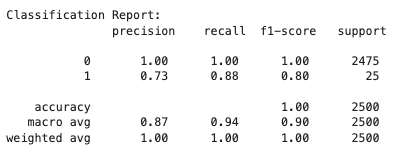
\includegraphics[width=0.6\textwidth]{figures/svm_results.png}
\end{figure}

Figure 9 shows the estimated feature importances of the predictors used by the SVM model via their permutation importance scores: 

\begin{figure}[h!]
    \centering
    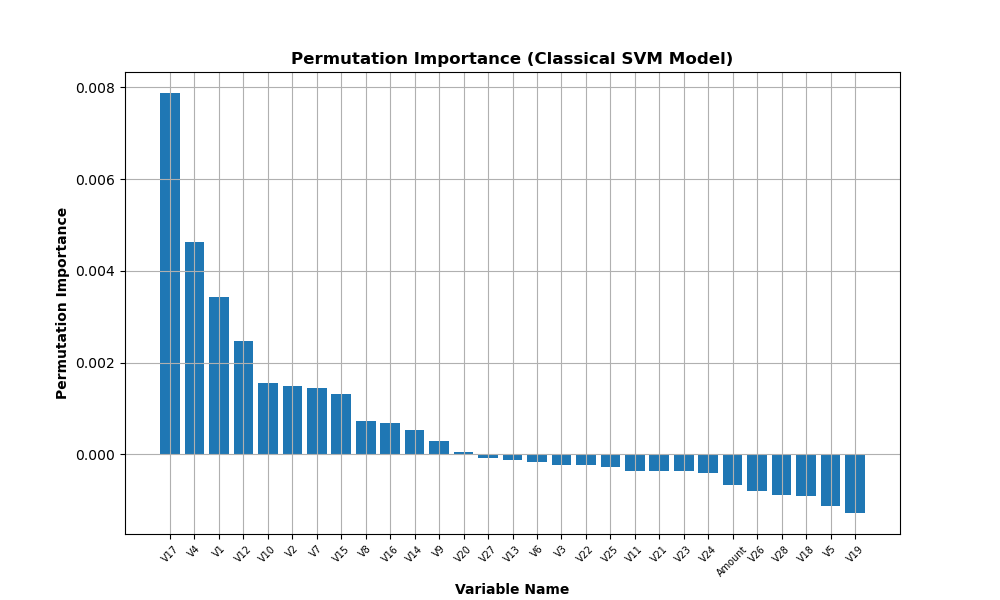
\includegraphics[width=1\textwidth]{figures/fig_9.png}
    \captionsetup{font=small} 
    \caption{Permutation importance of all predictors using the best performing SVM model.}
    \label{fig9}
\end{figure}


% -----------------------------------------------------------Results: Classical ML Algorithms: Random Forest-------------------------------------------------------------------------------------------


\subsubsection{RF}

Table 4 below is an updated version of table 2 that shows the values of the hyperparameters that resulted in the most successful RF model:

\begin{table}[h!]
    \centering
    \begin{tabular}{|c|c|c|}
        \hline
        \textbf{Hyperparameter} & \textbf{Candidates} & \textbf{Selection}\\ \hline
        $\texttt{n\_estimators}$ &  100, 200 & 100 \\ \hline
        $\texttt{max\_depth}$ & 10, 20 & 10\\ \hline
        $\texttt{min\_samples\_split}$ & 5, 10 & 5\\ \hline
        $\texttt{min\_samples\_leaf}$ & 1, 2 & 1 \\ \hline
    \end{tabular}
    \caption{An updated version of Table 2 that shows the value of the hyperparameters from the most successful SVM model}
    \label{tab4}
\end{table}


This model was then used to make predictions on the test set, producing the following results:

\begin{figure}[h!]
	\centering
	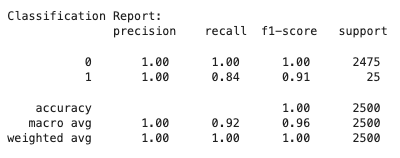
\includegraphics[width=0.6\textwidth]{figures/rf_results.png}
\end{figure}

Figure 10 shows the estimated feature importances of the predictors used by the RF model: 

\begin{figure}[h!]
    \centering
    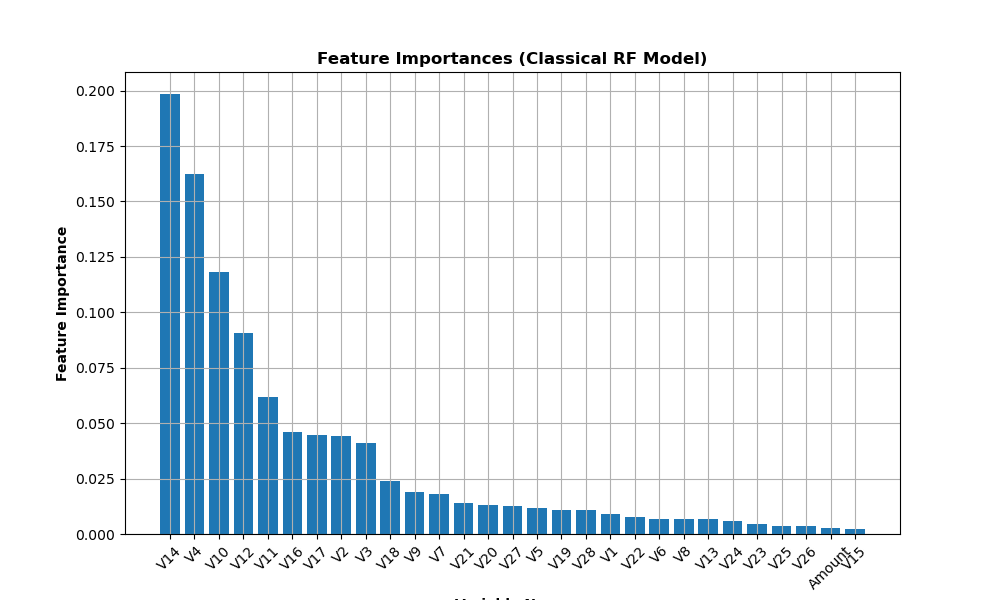
\includegraphics[width=1\textwidth]{figures/fig_10.png}
    \captionsetup{font=small} 
    \caption{Feature importance of all predictors using the best performing SVM model.}
    \label{fig10}
\end{figure}


% -----------------------------------------------------------Results: QML Algorithms: QSVM-------------------------------------------------------------------------------------------


\subsection{QML Algorithms}
\subsubsection{QSVM}

Figure 11 shows a summary of the fitting runtimes for the different quantum circuits tested:

\begin{figure}[h!]
    \centering
    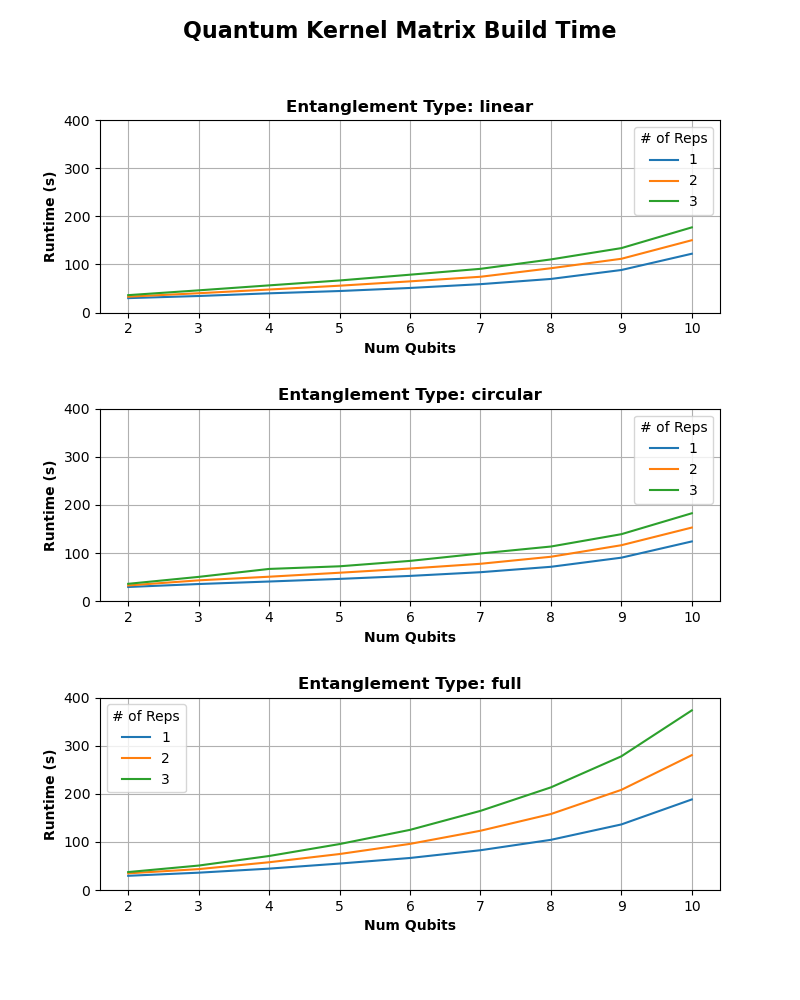
\includegraphics[width=1\textwidth]{figures/fig_11.png}
    \captionsetup{font=small} 
    \caption{Fitting runtimes for the QSVC function using as a function of the number of qubits, reps, and entanglement patterns.}
    \label{fig11}
\end{figure}

Further evaluation of these fitting runtimes $F$ revealed that they maintain a linear relationship with the number of repetitions $R$, and a non-linear second polynomial relationship with the number of qubits $n$:

\begin{equation}
F \propto R \cdot n^2
\end{equation}

Figure 11 shows that proportionality defined in Equation 19 was observed across all entanglement types, however models using full entanglement patterns exhibited longer runtimes compared to those with linear or circular structures (especially as the number of repetition and qubits increases). To assist in modeling the effect of entanglement pattern on the fitting runtime, the total number of quantum gates or quantum operations $G$ in each circuit was calculated. Determining $G$ requires determining the number of operations stemming from both the quantum entanglement and rotation transformations:

\begin{itemize}
	\item \textbf{For linear patterns}: $G=R(n-1 + n) = R(2n-1)$. \\ \textbf{Explanation:} $n-1$ gates from entanglement (gates exist between the first and second qubits, the second and third qubits, etc), $n$ rotation gates, multiplied by the number of repetitions.
	\item \textbf{For circular patterns:} $G=R(n + n) = 2Rn$. \\ \textbf{Explanation:} Same as linear with an added entanglement gate between the first and last qubit.
	\item \textbf{For full patterns:} $G=R(\frac{n(n-1)}{2} + n) = R\cdot \frac{n^2+n}{2}$. \\ \textbf{Explanation:} Same as linear and circular but there are $\frac{n(n-1)}{2}$ entanglement gates (each qubit has a gate between all other qubits). 
\end{itemize}

Based off the results shown in Figure 12, the fitting times of the QSVC models follow an near perfect linear pattern, meaning the time to execute each of the quantum transformations in a circuit are nearly identical.  

\begin{figure}[h!]
    \centering
    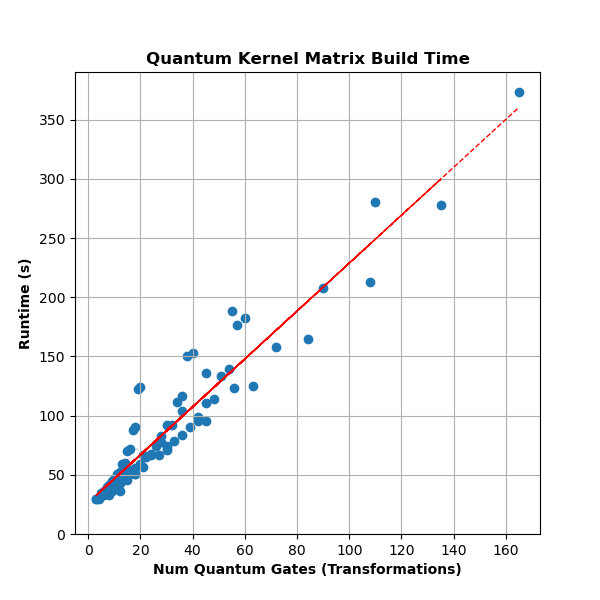
\includegraphics[width=0.6\textwidth]{figures/fig_12.png}
    \captionsetup{font=small} 
    \caption{Fitting runtimes for the QSVC function using as a function of the number of quantum gates in the circuit. Based on the slope of the linear fit, each operation takes an average of 1.88s.}
    \label{fig12}
\end{figure}

Figure 13 shows how the F1 scores of the fraudulent class differ when using different quantum circuits:


\begin{figure}[h!]
    \centering
    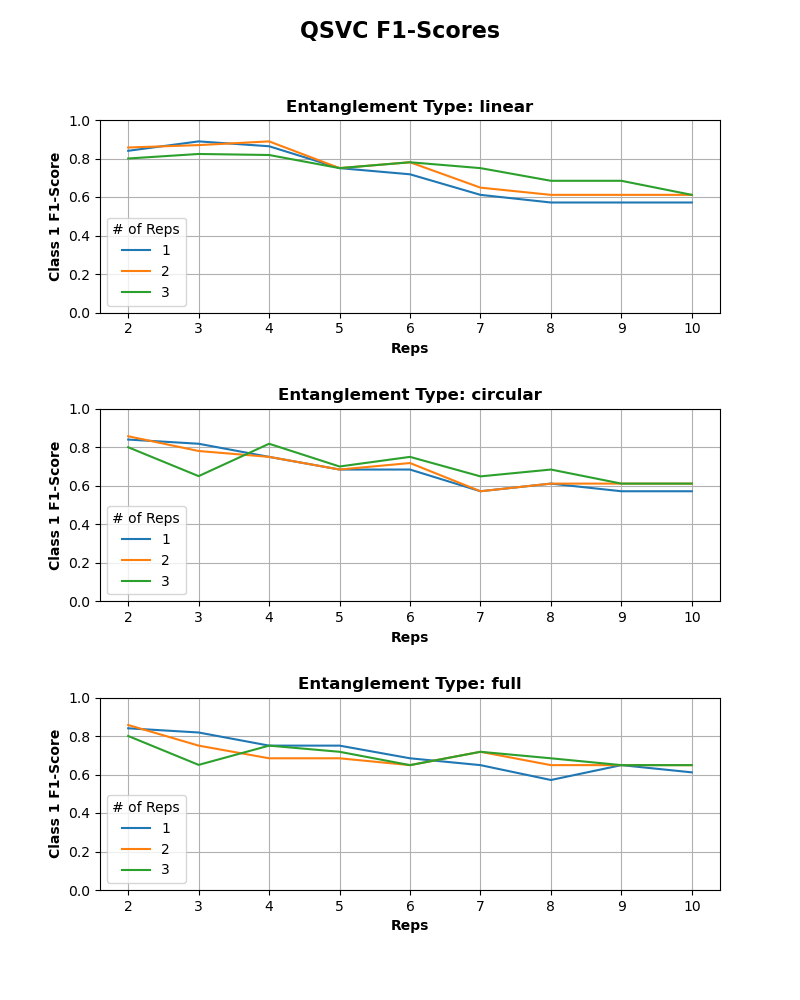
\includegraphics[width=1.0\textwidth]{figures/fig_13.png}
    \captionsetup{font=small} 
    \caption{Testing data F1 scores achieved on the fraudulent class using the QSVC function as a function of the number of qubits, reps, and entanglement patterns.}
    \label{fig13}
\end{figure}

\newpage

\section{References}

\begin{enumerate}
    \item \href{https://journals.aps.org/pra/abstract/10.1103/PhysRevA.58.915}{E. Farhi, and S. Gutmann, ``Quantum computation and decision trees,” \textit{Physical Review A}, \textbf{58}(2):915–928, 1998.}
    
    \item \href{https://arxiv.org/abs/1907.06840}{K. Khadiev, I. Mannapov, and L. Safina, ``The Quantum Version Of Classification Decision Tree Constructing Algorithm C5.0,” //\textit{arXiv} preprint arXiv:1907.06840, 2019.}
   
   \item \href{https://arxiv.org/abs/2112.13346}{K. Khadiev, and L. Safina, ``The Quantum Version of Prediction for Binary Classification Problem by Ensemble Methods,” //\textit{arXiv} preprint arXiv:2112.13346, 2021.}
   
   \item \href{https://arxiv.org/abs/2210.02355}{M. Srikumar, C.D. Hill, and Lloyd, ``A kernel-based quantum random forest for improved classification,” //\textit{arXiv} preprint arXiv:2210.02355, 2022.}
   
   \item \href{https://doi.org/10.1016/S0893-6080(03)00087-X}{D. Anguita, S. Ridella, F. Rivieccio, and R. Zunino, ``Quantum optimization for training support vector machines,” \textit{Neural Networks}, \textbf{16}(5-6):763–770, 2003.}
   
   \item \href{https://doi.org/10.26421/QIC17.15-16}{R. Chatterjee, and T. Yu, ``Generalized Coherent States, Reproducing Kernels, and Quantum Support Vector Machines,” \textit{Quantum Information \& Computation}, \textbf{17}(15-16), 2017.}
   
   \item \href{https://doi.org/10.1038/nature23474}{J. Biamonte, P. Wittek, N. Pancotti, P. Rebentrost, N. Wiebe, and S. Lloyd, ``Quantum machine learning,” \textit{Nature}, \textbf{549}(7671):195–202, 2017.}
   
   \item \href{https://doi.org/10.3390/e25020287}{A. Zeguendry, Z. Jarir, and M. Quafafou, ``Quantum Machine Learning: A Review and Case Studies,” \textit{Entropy}, \textbf{25}(2):287, 2023.}
   
   \item \href{https://doi.org/10.21203/rs.3.rs-1434074/v1}{S. Zheng, J. Guo, X. Ding, X. Zhou, J. Wang, H. Lian, Y. Gao, B. Zhao, and J. Xu, “Demonstration of Breast Cancer Detection Using QSVM on IBM Quantum Processors,” //\textit{Research Square} preprint researchsquare:10.21203, 2022.}
   
   \item \href{https://doi.org/10.48550/arXiv.2408.04543}{Z.J. Luo, T. Stewart, M. Narasareddygari, R. Duan, and S. Zhao, “Quantum Machine Learning: Performance and Security Implications in Real-World Applications,” //\textit{arXiv} preprint arXiv:2408.04543, 2024.}
   
   \item \href{https://doi.org/10.22331/q-2023-11-29-1191}{E.A. Cherrat, S. Raj, I. Kerenidis, A. Shekhar, B. Wood, J. Dee, S. Chakrabarti, R. Chen, D. Herman, S. Hu, P. Minssen, R. Shaydulin, Y. Sun, R. Yalovetzky, and M. Pistoia, “Quantum Deep Hedging,” \textit{Quantum} 7:1191, 2023.}
   
   \item \href{https://doi.org/10.34190/eccws.23.1.2258}{T. Nguyen, T. Sipola, and J. Hautamäki, “Machine Learning Applications of Quantum Computing: A Review,” \textit{European Conference on Cyber Warfare and Security}, \textbf{23}(1):322–330, 2024.}
   
   \item \href{https://doi.org/10.1142/S0219749923500442}{N. Innan, M.A.-Z. Khan, and M. Bennai, “Financial Fraud Detection: A Comparative Study of Quantum Machine Learning Models,” \textit{International Journal of Quantum Information} \textbf{22}(2):2350044, 2024.}
   
   \item \href{https://doi.org/10.48550/arXiv.2208.01203}{O. Kyriienko, and E.B. Magnusson, “Unsupervised quantum machine learning for fraud detection,” //\textit{arXiv} preprint arXiv:2208.01203, 2022.}
   
   \item \href{https://thequantuminsider.com/2024/07/19/deloitte-italy-explores-quantum-machine-learning-for-digital-payments-fraud-detection/}{M. Swayne, “Deloitte Italy Explores Quantum Machine Learning for Digital Payments Fraud Detection,” \textit{The Quantum Insider}, 2024.}
   
   \item \href{https://www.kaggle.com/datasets/nelgiriyewithana/credit-card-fraud-detection-dataset-2023}{Nidula Elgiriyewithana, “Credit Card Fraud Detection Dataset 2023,” www.kaggle.com, 2023.}
   
   \item \href{https://www.eba.europa.eu/sites/default/files/2024-08/465e3044-4773-4e9d-8ca8-b1cd031295fc/EBA_ECB\%202024\%20Report\%20on\%20Payment\%20Fraud.pdf}{European Banking Authority, ``2024 Report on Payment Fraud", 2024.}
   
   \item \href{https://books.google.com/books/about/Exploratory_Data_Analysis.html?id=UT9dAAAAIAAJ}{J.W. Tukey, ``Exploratory Data Analysis," (Addison-Wesley Pub. Co, Reading, Mass., 1977).}
   
   \item \href{https://doi.org/10.1214/aoms/1177730388}{C. Hastings, F. Mosteller, J.W. Tukey, and C.P. Winsor, ``Low Moments for Small Samples: A Comparative Study of Order Statistics,” \textit{The Annals of Mathematical Statistics}, \textbf{18}(3):413–426, 1947.}
   
   \item \href{https://www.nature.com/articles/s41592-019-0686-2}{P. Virtanen, et. al., “SciPy 1.0: fundamental algorithms for scientific computing in Python,” \textit{Nature Methods}, \textbf{17}(3):261–272, 2020.}
   
   \item \href{https://doi.org/10.2307/2334522}{D’Agostino, R. B., ``An omnibus test of normality for moderate and large sample size”, \textit{Biometrika}, 58:341-348, 1971.}
   
   \item \href{https://doi.org/10.2307/2335012}{D’Agostino, R. and Pearson, E. S., ``Tests for departure from normality”, \textit{Biometrika}, 60:613-622, 1973.}
   
   \item \href{https://doi.org/10.1093/biomet/87.4.954}{I.-K. . Yeo, “A new family of power transformations to improve normality or symmetry,” \textit{Biometrika} \textbf{87}(4):954–959, 2000.}
   
   \item \href{https://doi.org/10.2307/2331554}{Student, “The Probable Error of a Mean,” \textit{Biometrika}, \textbf{6}(1):1, (1908).}
   
   \item \href{https://link.springer.com/book/10.1007/978-1-4757-3264-1}{Vladimir Naoumovitch Vapnik, ``The Nature of Statistical Learning Theory," (Springer, Cop, New York, 2000).}
   
   \item \href{https://doi.org/10.1023/A:1010933404324}{24 L. Breiman, ``Random Forests,” Machine Learning 45(1), 5–32 (2001).}
   
   \item \href{https://www.ibm.com/quantum/pricing}{``IBM Quantum Computing | Pricing,” www.ibm.com.}
   
   \item \href{https://doi.org/10.48550/arXiv.2405.08810}{A. Javadi-Abhari, et. al., ``Quantum computing with Qiskit,” //\textit{arXiv} preprint arXiv:2405.08810, 2024.}
   
   \item \href{https://doi.org/10.1613/jair.953}{N.V. Chawla, K.W. Bowyer, L.O. Hall, and W.P. Kegelmeyer, ``SMOTE: Synthetic Minority Over-sampling Technique,” \textit{Journal of Artificial Intelligence Research}, \textbf{16}(16):321–357, 2002.}
\end{enumerate}









\end{document}